\documentclass[main.tex]{subfiles}

\begin{document}
\section{Methodology} \label{methodology}

In this section we describe the techniques we considered, brainstormed during the project and those that are implemented. \autoref{summary_table} is an effort to summarise all these techniques, but they are not exhausive. This is because we realised that the order of applying these techniques will have varying impact on subsequent stages of the task. To further complicate the matter, filtering the images with a gaussian filter, median filter, or 'morphing' the images with a structuring element (such as a disk with 15 pixels) before or after each stage in the pipeline will have varying impact to the outcome. The number of permutation in these steps is too large for us to consider all. What we have implemented is not the optimum, but one of the many options. We rationalise the choice of parameters along the course of this section.

The reader should refer to \hyperlink{training}{training.m}, \hyperlink{imageprocessing}{image\_processing.m}, \hyperlink{extractfeat}{extract\_features.m}, \hyperlink{manclf}{manual\_classification.m}, and  \hyperlink{trainclf}{trainclf\_loglikelihood.m}.

%  >{\centering}m{5cm}
\begin{table}[!h]
\begin{center}
  \begin{tabular}{p{2.22cm}|p{2.2cm}|p{.5\textwidth}| p{1.5cm} }
    % >{\centering}m{1cm} | >{\centering}m{1cm} | >{\centering}m{1cm} | >{\centering}m{1cm} }
    \toprule
    Task            & Subtask      & Techniques &     Implmentation \\
    \midrule
    Image Processing & Background Model & Finding median for each pixel and each channel & \checkmark \\
    {}  &  {} &   Finding median of neighbourhood for each pixel and each channel & \checkmark \\
    {} & {} & Probabilistic Modeling of background & {} \\
    \hline
    {} & Thresholding & Finding minimum of bimodal distribution & \checkmark \\
    {} & {} & Otsu's method for thresholding & {} \\
    {} & {} & Using Gradient magnitude of image & {} \\
    \hline
    Feature Extraction  & Global Descriptors &
    \begin{itemize}[noitemsep,topsep=0pt,parsep=0pt,partopsep=0pt]
      \item Area
      \item Perimeter
      \item Compactness
      \item Rectangularity
      \item Elongation
    \end{itemize} & \checkmark \\
    \hline
    {} & Moments             &
    \begin{itemize}[noitemsep,topsep=0pt,parsep=0pt,partopsep=0pt]
      \item Hu's Invariant moments\newline(7 features)
      \item Complex moments\newline(6 features)
    \end{itemize}& \checkmark \\
    \hline
    Classification & - & Multivarate Gaussian Model & \checkmark \\
    {}             & {} & Linear Discriminant & {}\\
    \bottomrule
  \end{tabular}
\end{center}
\caption{Summary of techniques in Coinsy.}
\label{summary_table}
\end{table}

% ====================================================================== %
\subsubsection*{Normalisation and Background Modelling}
In this coursework, since a background image is not readily available, we have to model it. Noting that images varies in illumination, we have to make the images comparable by normalising it first, using the following formula.
$$ P_{r,c}(R',G',B')=(\frac{R}{\sqrt(R^2+G^2+B^2)},\frac{G}{\sqrt(R^2+G^2+B^2)},\frac{B}{\sqrt(R^2+G^2+B^2)})$$
This is executed by \hyperlink{normRGB}{normalise\_RGB.m}.The outcome of the background with and without normalisation is shown in \autoref{bg_model}.

\begin{figure}[!h]
  \centering
  \begin{subfigure}[b]{.45\textwidth}
    \centering
    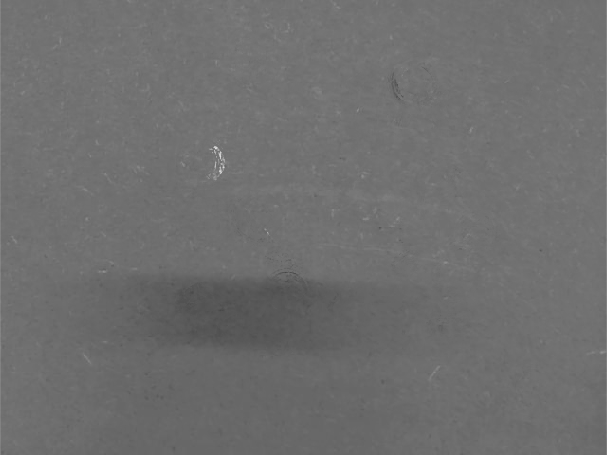
\includegraphics[width=\textwidth]{./img/bg_model/org_1.png}
    \caption{Background model without normalisation}
  \end{subfigure}
  \begin{subfigure}[b]{.45\textwidth}
    \centering
    
\includegraphics[width=\textwidth]{./img/bg_model/norm_1.png}
    \caption{Background model after normalisation}
  \end{subfigure}
  \caption{Background model generated from all 14 images.}
  \label{bg_model}
\end{figure}

Next, with objects scattered around randomly in the images, we find the median of all image pixels for each channel separately in order to reconstruct the background.
Our approach uses a neighbourhood of pixels for each pixel in the backgrund model. Hence, for a window of size 3, we have
$bg\_model_{r,c} = median(i_{r+1,c+1}, i_{r+1,c}, i_{r+1,c-1},
                          i_{r,c+1}, i_{r,c}, i_{r,c-1},
                          i_{r-1,c+1}, i_{r-1,c}, i_{r-1,c-1}) $.

The outcomes of the background (with and without normalisation) with different neighbourhood size = $1$, $3$, $5$ are shown in \autoref{montage_bg}. This appraoch requires large amount of memory and time to compute the background model. We find that although the images have subtle differences, the subimages we derieved in the later part of the pipeline is actually better.

\begin{figure}[!h]
  \centering
  \begin{subfigure}[t]{\textwidth}
    \centering
    \begin{subfigure}[t]{.3\textwidth} %% taking median
        \centering
        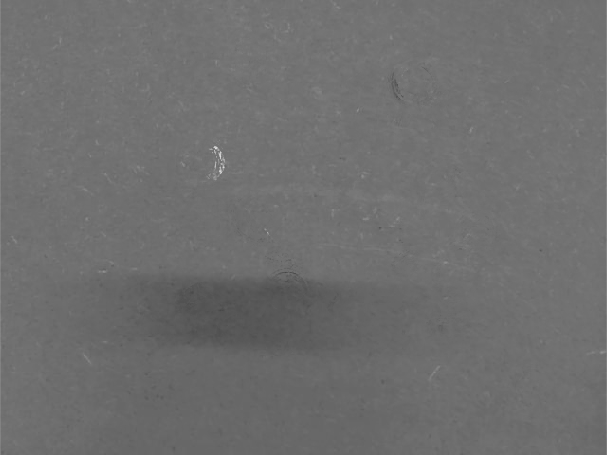
\includegraphics[width=\textwidth]{./img/bg_model/org_1.png}
    \end{subfigure}
    \begin{subfigure}[t]{.3\textwidth} %% window_size = 3
        \centering
        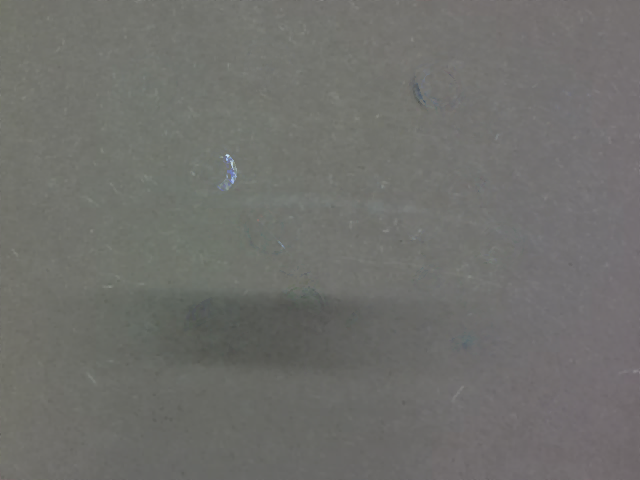
\includegraphics[width=\textwidth]{./img/bg_model/org_3.png}
    \end{subfigure}
    \begin{subfigure}[t]{.3\textwidth} %% window_size = 5
        \centering
        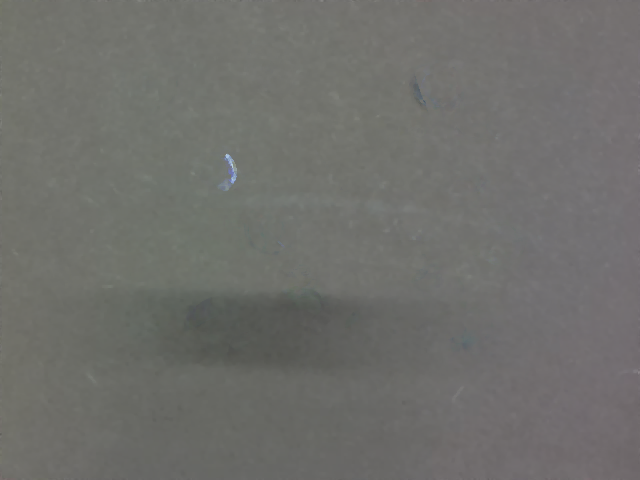
\includegraphics[width=\textwidth]{./img/bg_model/org_5.png}
    \end{subfigure}
  \end{subfigure} %% LOWER IMAGE - NORMALISED
  \begin{subfigure}[b]{\textwidth}
    \centering
    \begin{subfigure}[t]{.3\textwidth} %% taking median
        \centering
        
\includegraphics[width=\textwidth]{./img/bg_model/norm_1.png}
        \caption{Neighbouhood=1}
    \end{subfigure}
    \begin{subfigure}[t]{.3\textwidth} %% window_size = 3
        \centering
        
\includegraphics[width=\textwidth]{./img/bg_model/norm_3.png}
        \caption{Neighbourhood=3}
    \end{subfigure}
    \begin{subfigure}[t]{.3\textwidth} %% window_size = 5
        \centering
        
\includegraphics[width=\textwidth]{./img/bg_model/norm_5.png}
        \caption{Neighbourhood=5}
    \end{subfigure}
  \end{subfigure}
  \caption{Background extraction with different neighbourhood size.}
  \label{montage_bg}
\end{figure}


The sample images with their background removed is shown in \autoref{montage_data_bgremove}. This removal process: $img\_bg\_removed_{r,c}(R,G,B) = img_{r,c}(R,G,B) - bg\_model_{r,c}(R,G,B)$ , however, also inevitably reduce the intensity for the bottom half of each images, such that the objects are no longer salient. This is because the background we modelled have a lower intensity at the bottom, possibly due to presence of shadow in all 14 images.

An alternative approach we considered is to find the average of the neighbourhood. However, we did not materialise this, as the presence of high pixel intensity (such as in the presence of an object in the foreground) will distort the mean, giving an inaccurate representation of the background.

%% Can consider include historgram to show the effect?
% Nevertheless, the historgram  is still bimodal, which is essential for thresholding to be effective.
% ====================================================================== %

\subsubsection*{Segmentation}
After the background is removed, the objects are left in the image. Our next task is to extract these regions where the objects exists. We used \hyperlink{dothresh}{dothresh.m} on each image to:
\begin{enumerate}
  \item Find the histogram of the pixel intensity
  \item Find the threshold of the histogram - \texttt{thresh}
  \item Apply this threshold value to the image\\(i.e. $if$ $IMG_{i,j} \ge thresh$, $IMG_{r,c,chn} = 1,$ $else$ $ IMG_{r,c,chn} = 0$
  \item Produce a binary image, \texttt{BW}, using:$$BW_{r,c} = IMG_{r,c,R} || IMR_{r,c,G} || IMG_{r,c,B}$$
\end{enumerate}

The binary image indicates the existence of objects as 1 (white) and the background as 0 (black). \autoref{} are the binary images for the sample images.

%% INSERT IMAGE HERE!

This thresholding algorithm works fine when the histogram produced is bimodal. However,
% ====================================================================== %
\subsubsection*{Filtering}


\subsection{Classification}





\end{document}
